\section{Optimization system}
\label{sec:os_implementation}

Given a FTP request, the Optimization System (OS) is the module that determines the respective solutions, using the strategies described in subsection \ref{sec:os_design}. This module was implemented using the Python3 programming language, and uses the \textit{numpy} library \cite{numpy} for the construction and management of the multi-dimensional (and often very large) arrays, which describe an FTP instance. 

The developed optimization system implements each of the three proposed optimization strategies: the nearest neighbour heuristic, the ACO and the SA metaheuristics (section \ref{sec:meta}). The adopted implementation of the nearest neighbour algorithm closely follows its definition. Consequently, it decided not to discuss it here. Instead, this subsection will focus on the implementation details of the ACO and the SA metaheuristics.

The implementation of the ACO follows the methodology described in subsection \ref{sec:aco} and is illustrated in figure \ref{fig:aco_flow}. This metaheuristic receives, as input, a data structure describing the FTP requests, which includes the weight matrix  and the constraints of the problem. This metaheuristic starts by initializing the algorithmic specific parameters, using the values presented in table \ref{tab:parameters}. 
It is also necessary to initialize the pheromone matrix, by setting each entry to a value defined by equation \ref{eq:tau_zero}.
%It also requires the initialization of the pheromone matrix, by initializing each entry to a value calculated using equation \ref{eq:tau_zero}. 

\begin{table}[t]
\centering
\caption{Algorithm specific parameters.}
\label{tab:parameters}
\begin{tabular}{c l c}
\hline
Alg.    &           Parameter         &       Value \\ \hline
%\multirow{2}{*}{FTP}    &           Cost weight ($w_p$)               &         0.7 \\
%                        &           Duration weight ($w_d$)               &         0.3 \\ \hline 
\multirow{5}{*}{ACO}    &           Pheromone relative influence ($\alpha$)              &         1 \\
                        &           Heuristic relative influence ($\beta$)               &         5 \\
                        &           Pheromone evaporation rate ($\rho$)                  &       0.1 \\
                        &           Exploration rate ($Q_0$)                  &       0.9 \\ 
                        &           Number of ants ($m$)                     & 10 \\ \hline
\multirow{6}{*}{SA}     &           First iter. acceptance prob. ($p_0$)                   & 0.98  \\ 
                        &           Last iter. acceptance prob. ($p_f$)                   & $10^{-300}$  \\
                        &           Initial temperature ($t_0$)                   & see Eq.~\ref{eq:t_zero} \\
                        &           Final temperature ($t_f$)                   & see Eq.~\ref{eq:cooling}  \\
                        &           Cooling parameter ($\lambda$)               & see Eq.~\ref{eq:lambda} \\
                        &           Markov chain length ($M$)                     & $N$ \\ \hline
                         
\end{tabular}
\end{table}



\begin{figure}[h]
  \centering
  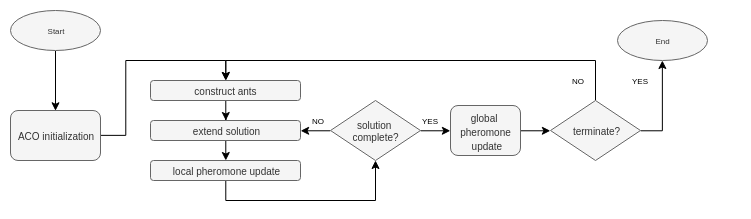
\includegraphics[width=\textwidth]{./Figures/system_implementation/aco_flow.png}
  \caption{Flowchart of the implemented Ant Colony System procedure.}
  \label{fig:aco_flow}  
\end{figure}

This is followed by the initialization of all ants belonging to the colony. Each ant is implemented as an independent thread, which allows for the colony to run in parallel. Thus, all ants construct a solution to the problem in an autonomous way, using the transition rules described in equations \ref{eq:selection_rule}, \ref{eq:exploitation} and \ref{eq:exploration}. At each step of the construction process, it is necessary to apply a local pheromone update, by using equation \ref{eq:local_update}, which decreases the probability of that solution component being selected by other ants, in the same iteration. After each ant finishes the construction of a solution, it is necessary perform the pheromone update (equation \ref{eq:pheromone_update}), as to reflect the search experience. Given that each ant is an independent thread, it is necessary to lock the pheromone matrix, as to protect it from being accessed and manipulated by multiple threads at the same time.

In its turn, the implementation of the SA follows the methodology described in subsection \ref{sec:sa}, as it is illustrated in figure \ref{fig:sa_flow}. As it happens with the ACO, the SA metaheuristics receives as input the relevant data to describe the FTP, and initializes its algorithmic specific parameters according to table \ref{tab:parameters}. This is followed by the determination of the cooling schedule. To do so, it is necessary to construct a number of solutions, as to calculate the average difference in the objective function, which allows the calculation of the initial temperature (equation \ref{eq:t_zero}) and cooling parameter (equation \ref{eq:lambda}). 

\begin{figure}[h]
  \centering
  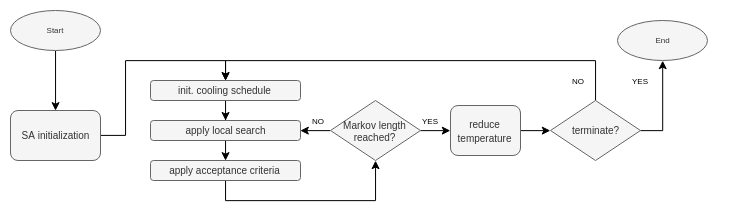
\includegraphics[width=\textwidth]{./Figures/system_implementation/sa_flow.png}
  \caption{Flowchart of the implemented Simulated Annealing procedure.}
  \label{fig:sa_flow}  
\end{figure}

%After this initialization process, the SA metaheuristics starts the optimization process by generatinga candidate solution, by applying a local search procedure (2-opt) to the current solution. To accept thissolution, it is necessary to apply the Metropolis acceptance criteria (equation 3.10). This process, calledMarkov cycle, is repeated for a given number of times.  Unlike the ACO implementation, the solutionconstruction process of the implemented SA follows a serial approach.  After each Markov cycle, thetemperature of the system is reduced, by applying equation 3.11.  As the temperature decreases, thealgorithm becomes increasingly greedy and converges to a local optimum.

%After this initialization process, the SA metaheuristics starts the optimization process by generating a candidate solution, by applying a
%2-opt move, described in section \ref{sec:local_search}, to the current solution.
%local search procedure (2-opt move, described in section \ref{sec:local_search}) to the current solution. 
%To accept this solution, it is necessary to apply the Metropolis acceptance criteria (equation \ref{eq:metropolis}). This two step process, called Markov cycle, is repeated for a predefined number of times (see table \ref{tab:parameters}). Unlike the ACO implementation, in which the the solution construction process is parallel, the developed Markov cycle follows a serial approach. After completing a cycle, the temperature of the system is reduced, by applying equation \ref{eq:cooling}. As the temperature decreases, the algorithm becomes increasingly greedy and converges to a local optimum.

After this initialization step, the SA system starts the optimization cycle, by constructing a new candidate solution $y$ based on the current solution $x$, using a 2-opt move, as described in section \ref{sec:local_search}.
%, to the current solution.
%local search procedure (2-opt move, described in section \ref{sec:local_search}) to the current solution. #
To accept the candidate solution $y$, it is necessary to apply the Metropolis acceptance criteria (see equation \ref{eq:metropolis}).
Unlike the ACO implementation, in which the the solution construction process is parallel, the developed Markov cycle follows a serial approach, given that the candidate solution $y$ is always constructed based on the current solution $x$. If there were multiple threads constructing solutions at the same time, the current solution would be an uncertain entity.
After completing a cycle, the temperature of the system is reduced, by applying equation \ref{eq:cooling}. As the temperature decreases, the algorithm becomes increasingly greedy and converges to a local optimum.

%This two step process, called Markov cycle, is repeated for a predefined number of times (see table \ref{tab:parameters}). Unlike the ACO implementation, in which the the solution construction process is parallel, the developed Markov cycle follows a serial approach. After each cycle, the temperature of the system is reduced, by applying equation \ref{eq:cooling}. As the temperature decreases, the algorithm becomes increasingly greedy and converges to a local optimum.


Both metaheuristics have a stop-criteria that is evaluated at the end of each solution construction cycle (the ants construction procedure, and the Markov cycle). This criteria is either set to a maximum number of iterations, or to a maximum allowable execution time. When the stop-criteria is reached, these heuristics return the best solution found so far. 

It is worth noting that the solution returned by the ACO and the SA modules correspond to a set of solution components 
%($a_{0, i}, a_{i, i+1}, \dots, a_{n, n+1}$)
, which define both the pair of cities and the schedule of the arc traversal. If the problem under resolution is a user request issued by the CSA, it is necessary to construct the set of flights which characterize the solution to the FTP request. Thus, the SSA must map each solution component to a particular flight, as to produce the itinerary for the requested trip. 


% \begin{table}[t]
% \centering
% \caption{Algorithm specific parameters.}
% \label{tab:parameters}
% \begin{tabular}{c l c}
% \hline
% Alg.    &           Parameter         &       Value \\ \hline
% %\multirow{2}{*}{FTP}    &           Cost weight ($w_p$)               &         0.7 \\
% %                        &           Duration weight ($w_d$)               &         0.3 \\ \hline 
% \multirow{5}{*}{ACO}    &           Pheromone relative influence ($\alpha$)              &         1 \\
%                         &           Heuristic relative influence ($\beta$)               &         5 \\
%                         &           Pheromone evaporation rate ($\rho$)                  &       0.1 \\
%                         &           Exploration rate ($Q_0$)                  &       0.9 \\ 
%                         &           Number of ants ($m$)                     & 10 \\ \hline
% \multirow{6}{*}{SA}     &           First iter. acceptance prob. ($p_0$)                   & 0.98  \\ 
%                         &           Last iter. acceptance prob. ($p_f$)                   & $10^{-300}$  \\
%                         &           Initial temperature ($t_0$)                   & see Eq.~\ref{eq:t_zero} \\
%                         &           Final temperature ($t_f$)                   & see Eq.~\ref{eq:cooling}  \\
%                         &           Cooling parameter ($\lambda$)               & see Eq.~\ref{eq:lambda} \\
%                         &           Markov chain length ($M$)                     & $N$ \\ \hline
                         
% \end{tabular}
% \end{table}

